\section{Approach}

The main objective of our approach was to determine the symbolic constraints of a program's execution path. The generated symbolic constraints give us a a way to generate input that will exercise the paths of the program. Using this information our technique aims to generate more tests. We generate more tests by looking at the constraints satisfied by a trace and negating the most recent constraint that hasn't been negated to generate test input that will take a different path. This process can be repeated until all satisfiable paths have been explored. 

The workflow of our technique is shown in Figure~\ref{fig:attributes}. Our approach starts by taking the original program and passing it through our transformation. This transformation is described below in Section~\ref{sec:dynamic}. The transformation instruments the original program with new instructions which evaluate and display the symbolic constraints of a program during execution. In order to determine if the instrumentation resulted in a program which was equivalent in terms of the control flow, a static control flow pass was also instrumented. The static control flow pass is described below in Section~\ref{sec:static}. The static pass went through a program and displayed all flow insensitive symbolic constraints from the program. This was done a check to ensure that dynamic transformation worked as expected.

We then executed the new program using random input. Using the symbolic constraints generated trace from the execution of the program using random inputs, we generate new input for the program. The new input is generated to explore new paths in the program under testing. We repeat this process until all paths have been executed. The final results will be a set of tests which explore different program paths and a set of constraints for the program describing each path through the program. 

\begin{figure}[t]
 \centering
 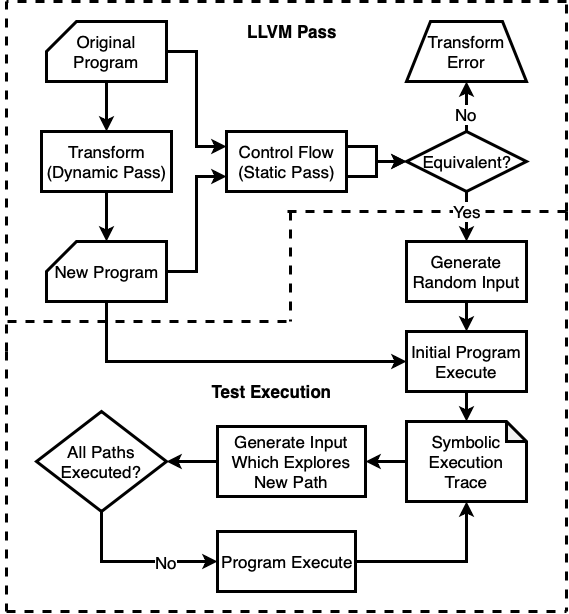
\includegraphics[width=\linewidth]{./images/overview.png}
 \caption{The general overview of our approach. Our approach starts by using LLVM's pass infrastructure to instrument the original program. We then execute the program using the symbolic execution trace to generate new inputs which drive the program on new paths.}
 \label{fig:attributes}
\end{figure}

\subsection{Dynamic Instrumentation Pass}
\label{sec:dynamic}

Our program transformation works as described in Algorithm~\ref{alg:dynamic_overview}. The algorithm takes an input $P$ which is the original program we want to run concolic testing on. The algorithm outputs $P'$: a new program which has been instrumented to output symbolic constraints of each predicate, the current variable values in each predicate and, whether the predicate final evaluation. The goal is transform $P$ to $P'$ while ensuring the control flow and decision points of both $P$ and $P'$ are equivalent.


\begin{algorithm}[t]
    \SetAlgoLined
    \SetKwProg{Fn}{Function}{}{}
    \SetKwFunction{overview}{General Overview}
    \SetKwInOut{KwIn}{Input}
    \SetKwInOut{KwOut}{Output}
    \KwIn{P}
    \KwOut{P'}

    about\_to\_branch = False\;
    P' = P\;

    \For {Each F in P}
    {
        \For {Each BB in P}
        {
            \For {Each I in P}
            {
                \If{I == Load\_Instruction}
                {
                    LHS = I.get\_LHS()\;
                    RHS = I.get\_RHS()\;
                    match\_vector = (LHS, RHS)\;
                }
                \If{I == Compare\_Instruction}
                {
                    op = I.get\_operands()\;
                    op\_m = match\_operands(op, match\_vector)\;
                    P'.log\_before(I, op\_m)\;
                    about\_to\_branch = True\;
                }
                \If{I == Branch\_Instruction}
                {
                    \If{about\_to\_branch}
                    {
                        about\_to\_branch = False\;
                        eval = evaluate\_results(I)\;
                        P'.log\_before(I, eval)\;
                    }
                }
            }
        }
    }
    
    return P'
 \caption{Dynamic Pass General Overview}
 \label{alg:dynamic_overview}
\end{algorithm}

Algorithm~\ref{alg:dynamic_overview} is an LLVM transformation pass. It works by first iterating through all functions $F$, then through all basic blocks $BB$ and then through all instructions $I$, shown in lines 3, 4 and 5 respectively. We then determine the type of instruction and handle each instruction differently. We are mainly interested in three instruction types namely, the load instruction, a compare instructions and a branch instruction as these instructions are used during program branching. The load instruction is important as it allows us to keep track of how local variables are transferred. The compare instruction compares two local variables, which determine the resulting flow of the program. Thus we are interested in obtaining the symbolic constraints from each of these compare instructions. The final instruction is the branch instruction. These instructions are where the branching actually occur in the program and thus an easy way to determine the result of a compare instruction is to evaluate the input to a branch instruction.  

Algorithm~\ref{alg:dynamic_overview} checks for a load instruction in line 6. If the instruction is indeed a load instruction the algorithm extracts the left hand side (LHS) in line 7 and right hand side (RHS) in line 8 from the instruction. The local variable in the RHS is being loaded into the local variable in the LHS. Thus we create a vector in line 9 which maps address and variables names of both sides. This mapping is used later during the constraints generation to determine which local variables are being used in each of the comparisons.

The next instruction Algorithm~\ref{alg:dynamic_overview} checks for is a compare instruction in line 11. The algorithm starts by getting the operands for the compare instruction in line 12. Using the load instructions vector, each of the operands are mapped to a known variable in line 13. Each of the operands are pass as arguments to a logging function which will display their values during a programs execution. Thus when a program is executed the constraints for each decision point in the program are printed out. Finally, line 15 sets a variable stating that a branch instruction is about to occur to true. 

The final instruction which is considered by the algorithm is a branch instruction as seen in line 17. The algorithm is only interested in branches which occur due to decision points such as compares. Other branch instructions are sometimes inserted into a program for instance to call a function. These do not change the flow of the program and so are ignored. Line 19 sets the $about\_to\_branch$ variable to false as the algorithm has found the expected branch instruction. Line 20 evaluates the result of the branch instruction. The result of this branch instruction is also the results of the compare instruction earlier. Finally algorithm~\ref{alg:dynamic_overview} prints the result of the branch instruction just before the branch occurs. Thus during execution our new program $P'$ at each decision point, we will print out the constraints containing references to known local variables and the results of each decision point will also be displayed.

\begin{algorithm}[t]
    \SetAlgoLined
    \SetKwProg{Fn}{Function}{}{}
    \SetKwFunction{overview}{General Overview}
    \SetKwInOut{KwIn}{Input}
    \KwIn{P}

    \For {Each F in P}
    {
        \For {Each BB in P}
        {
            \For {Each I in P}
            {
                \If{I == Load\_Instruction}
                {
                    LHS = I.get\_LHS()\;
                    RHS = I.get\_RHS()\;
                    match\_vector = (LHS, RHS)\;
                }
                \If{I == Compare\_Instruction}
                {
                    op = I.get\_operands()\;
                    op\_m = match\_operands(op, match\_vector)\;
                    op\_str = op\_m.to\_str()\;
                    display(op\_str)\;
                }
            }
        }
    }
 \caption{Static Pass General Overview}
 \label{alg:static_overview}
\end{algorithm}

\subsection{Static Pass}
\label{sec:static}

The static pass used an algorithm similar to the dynamic pass and is described in Algorithm~\ref{alg:static_overview}. There were however two major differences between the dynamic pass and that static pass. The first was that the static pass did not consider branching instructions. That is because the result of branching instructions can only be determined at runtime and thus is not applicable to a static pass. The second major difference is that the constraints are converted to a string representation in the static pass and displayed to the user. Thus no evaluation of the constraints takes place when the pass is run.


\subsection{Test Execution}

The process of generating and executing tests is described in Algorithm ~\ref{alg:input_testing}. To begin executing paths of the program, we first generate $n$ random values, one for each of the augmented program $P'$'s inputs as seen in lines 2 and 3. Next we create a list which will contain all the symbolic constraints found during program execution in line 5. While we have an input, $P'$ is run with these random inputs in lines 6 and 7. The program execution in line 7 returns a trace containing symbolic constraints for that specific run. This trace is appended to the list of constraints for all runs in line 8. Using the programs current trace and list of previous traces, we call a function solveConstraints which generates an input that will explore a new path in the program. Using this new input, we repeat the process until all paths have been found.

The function \textit{solveConstraints} in line 11 of Algorithm~\ref{alg:input_testing} is described as follows. First line 12 sets the input to NULL. If the constraints can not be solved this value will be returned and the concolic testing ended.  For each of the constraints in the program trace, we negate that constraint in line 14 by removing the last constraint, negating it and adding it back. If the new constraints have not been seen before, we pass them to an SMT solver which solves them and generates a new input, as shown in line 16. 

\begin{algorithm}[t]
    \SetAlgoLined
    \SetKwProg{Fn}{Function}{}{}
    \SetKwFunction{overview}{General Overview}
    \SetKwInOut{KwIn}{Input, n}
    \KwIn{P'}
    I = []\;
    \For{n times}{
        I[n] = random\_value()\;
    }
    constraints = []\;
    \While {I is not NULL}
    {
        trace = P'(I)\;
        constraints.append(trace)\;
        I = solveConstraints(trace, constraints)\;
    }
    
    \Fn{solveConstraints(T, SC)}{
        I' = NULL\;
        \For {Each t in size(T)}
        {
            new\_constraints = T - T[size(T)-t] + !T[size(T)-t]\;
            \If {new\_constraints not in SC}
            {
                I' = smt.solve(new\_constraints)\;
                break\;
            }
        }
        return I'\;
 }
    
 \caption{Input Testing Overview}
 \label{alg:input_testing}
\end{algorithm}